% !TEX root=template.tex

\typeout{NT FILE implementation.tex}

\prependtographicspath{{Chapters/Figures/}}

\glsresetall

%TODO: Maybe explain in way more detail the implementation? I can explain each agents implementation in more detail and add info on all the method? That feels excessive but it would increase page count I suspect

%O modelo de dados (?) todas as variáveis do programa desenvolvido

%Diagramas de classes com a implementação dos módulos e dos agentes

%Que interfaces existem entre os diferentes módulos, que dados são trocados nessas interfaces

%quais os métodos que são chamados quando uma sequência de execução de skill é feita

%quais os métodos quando um agente é lançado

%quais os behaviours utilizados para implementar os agentes

%quais as interações entre a tool que fizeste e o resto do ecossistema

%quais as libs que implementaste e como as fizeste (MQTT, HTTP, OPC UA)

\chapter{Implementation}
\label{cha:implementation}

Now that the proposed architecture of the system has been laid out and well defined, it is time to implement it. First the tools used are identified and each class was implementation is explained, their data models and methods. Then the different modules in the system that communicate through interfaces are identified, an explanation is done on how a human operator can interact with the system, what behaviours each agent makes use of and the developed \acrlongpl{LL} for hardware interfacing. Finally, the system operations and what behaviours and methods are called for each operation are also explained.\\

\section{System Implementation}
\label{sec:class_implementation}

The implementation needs to start with the deployment agents, since these are responsible for launching all other agent types. The \acrfull{DA} is tasked with deploying \acrfullpl{RA} and \acrfullpl{TA}. The \acrshort{DA} needs a \acrfull{GUI} to allow a user to launch these agents with the right configurations. These must include the agent type to be launched, the type of \acrlong{LL} the agent must use and its configurations. Like the \acrshort{DA}, the \acrfull{PM} also needs to launch agents, more specifically, \acrfullpl{PA}. This should also be done through a \acrshort{GUI} but this one should only show buttons per product type, and some information on the already deployed \acrshortpl{PA}.\\

The \acrshortpl{RA} and \acrshortpl{TA} will operate somewhat similarly to each other, with the \acrshortpl{RA} needing an extra step before a skill executes. They will register themselves in a registry of agents called the \acrfull{DF}. This \acrshort{DF} is the Yellow Pages Service mentioned in Chapter~\ref{cha:architecture}. This is mainly so that the \acrlongpl{PA} can find the right agent for the operation they need to accomplish. For skill execution, \acrshortpl{RA} and \acrshortpl{TA} are dependent on the \acrlong{ME}.\\\\

The \acrlongpl{PA} need to be constantly on a loop. They look at their production sequence and search for a \acrshort{RA} capable of performing the current skill. Upon finding it, they will request transportation to the station. Upon arrival, they will call for the skill to be performed on them. If the production sequence has been completed, they request transportation out of the production line. If not, the process must repeat until this condition is met.\\

The \acrlong{ME} will need to operate between the layers of agent and hardware. It needs to be able to use its configurations to load any developed \acrlong{LL}. It must also be capable of relaying messages from the agent to the hardware and vice versa. Multiple \acrlongpl{LL} need to be developed in order to test whether or not the \acrshort{ME} is capable of switching \acrshortpl{LL} during runtime.\\

\subsection{Implementation Tools}
\label{subsec:implementation_tools}

For the implementation of the \acrlong{ME} framework and accompanying \acrshort{MAS}, the Java programming language was selected, more specifically version 21.0.2 of the OpenJDK. As mentioned in \ref{subsec:best_practices_and_common_architectures}, \acrshort{JADE} was built with the \acrshort{FIPA} specifications in mind and its Java version is well supported, so this framework was chosen to implement the \acrlong{MAS}.

The \acrshort{JADE} framework provides a lot of tools for agent development, communication and management. It provides a lot of classes and methods useful for agent setup, communication, \acrshort{DF} registration and more. Since the Java language was going to be used for the \acrshort{MAS} and is one of the best supported in the world, the \acrlong{ME} and the \acrlongpl{LL} were also developed using it.\\

As mentioned in Chapter \ref{cha:architecture}, three main cyber-physical agent types were developed, \acrfullpl{RA}, \acrfullpl{TA} and \acrfullpl{PA}. Along with these, two more agents were created, \acrfull{PM} and \acrfull{DA}, with the purpose of launching and managing the other three agent types. All of these agents extend an interface "Agent" provided by \acrshort{JADE}.

This interface contains a lot of useful methods and variables, although not all of them are used in this \acrshort{MAS}. The methods used are the "setup" method, executed once when an agent is launched, and the "takeDown" method, executed when a agent is terminated. These methods must be overwritten to provide the agent with instructions on launch and termination.

Because the agents are launched through \acrshort{JADE}, the class constructor cannot have any initial arguments. To launch an agent with arguments, the method "getArguments" present in every agent can be used. It returns a generic object array a developer can then use to retrieve the arguments an agent is launched with.

\acrshort{JADE} also provides a lot of other classes that define agent behaviour. These classes must be defined inside the agents class to add new behaviours. Some of them must be used in order to make use of the different \acrshort{JADE} functionalities, like the \acrshort{FIPA} Contract Net. Others simply exist to add a bit more flexibility during development.\\

The behaviour classes used in this project were:
\begin{itemize}
	\item The "OneShotBehaviour" class, that adds a single behaviour to the agents behaviour sequence. It is executed once, and then is excluded from the sequence;
	\item The "ContractNetInitiator" class, that allows an agent to start interacting with other agents as the Initiator in the \acrshort{FIPA} Contract Net protocol. Once it finishes communications, it is excluded from the behaviour sequence;
	\item The "ContractNetResponder" class, that allows an agent to respond to messages as one of the Participants in the \acrshort{FIPA} Contract Net protocol; 
	\item The "AchieveREInitiator" class, that allows an agent to start interacting with anoter agent as the Initiator in the \acrshort{FIPA} Requests protocol. This class is also excluded from the behaviour sequence after communications are done;
	\item And the "AchieveREResponder" class, that allows an agent to respond to messages as a Participant in the \acrshort{FIPA} Requests protocol.
\end{itemize}

\subsection{Deployment Agent}
\label{subsec:deployment_agent}

Starting with deployment, the \acrlong{DA} was designed to allow a human user to deploy and terminate agents during the execution of the \acrshort{MAS}. In its constructor the functionalities of the \acrshort{GUI} are defined and some initial values are set. This class extends the "Agent" class, and only makes use of the "setup" method. All other functionalities are called on button presses, through events.

The "selectedAgent" field specifies which type of agent (\acrshort{RA} or \acrshort{TA}) is to be launched. This can be changed through a radio button on the interface.

The "xmlMarketplace" field is loaded during "setup" with the method "getMarketplaceLibraries", using the file pointed to by the "marketplaceXMLPath" String. It holds the path of the \acrshort{XML} file that contains the available \acrlongpl{LL}.

The "agentContainer" field holds a reference to the container where the agents deployed will be hosted. Finally, the "xmlConfigPath" is a user loaded value that is used to pass the \acrshort{LL} configurations file.\\

In Figure~\ref{fig:da_class_diagram}, some of the classes the agent uses to draw the \acrshort{GUI} are shown. These classes are part of the "javax.swing" package, useful to draw graphical interfaces. The "ContainerController", used to create a container where other agents are deployed, is a \acrshort{JADE} class. Also shown are the auxiliary "Constants" class, that stores constants useful for the correct operations of the \acrshort{MAS}. This class will be explained in more detail in Section~\ref{subsec:constants}.\\

\begin{figure}[h!]
	\centering
	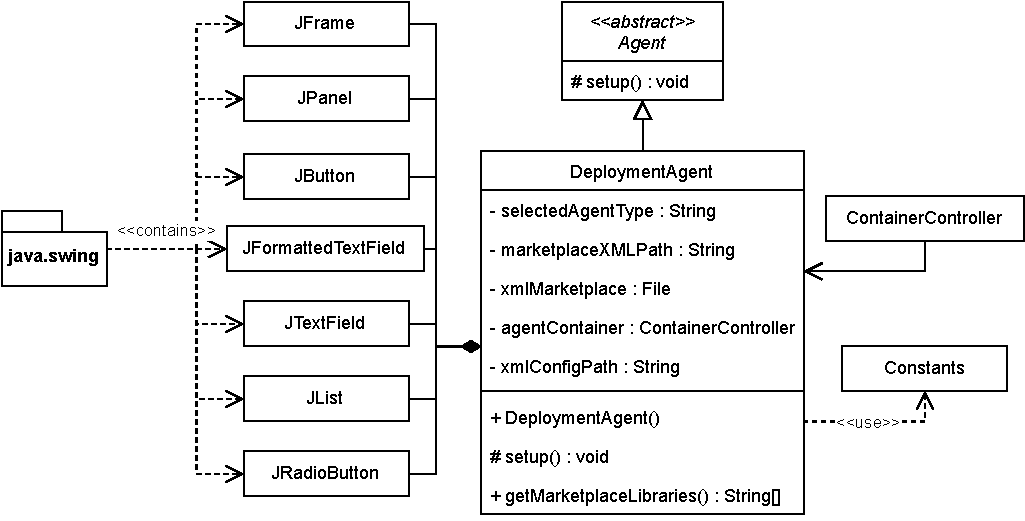
\includegraphics[scale=0.8]{DA_Class_Diagram}
	\caption{\acrlong{DA} class diagram.}
	\label{fig:da_class_diagram}
\end{figure}

\subsection{Resource Agent}
\label{subsec:resource_agent}

This agent is launched by the \acrshort{DA} because it is dependent on the parameters provided by it. The \acrlong{RA} class also extends the "Agent" abstract class, and overrides the "setup" and "takeDown" methods. It makes use of the "addBehaviour" and "getArguments" methods, as well as the "ContractNetResponder" and "AchieveREResponder" classes.

It makes use of the auxiliary "Constants" and "DFInteraction" classes, which will be explained in \ref{subsec:constants} and \ref{subsec:directory_facilitator}, respectively. It has two objects of type File called "xmlConfigFile" and "xmlMarketplaceFile", given as a parameter by the \acrshort{DA}, that store the corresponding files. The String "libType", also given as a parameter by the \acrshort{DA}, contains the type of \acrshort{LL} this agent is using and the String "location" contains the position of this agent in the physical system.\\

Finally, the object "moduleEngine" of type ModuleEngine holds the \acrshort{ME} instance this agent instantiates, and the ArrayList of Strings "associatedSkills" holds the list of all skills this agent is able to perform. This last object is initialized during setup, with the configurations provided by the \acrshort{DA} as well.\\

The "requestResponder" class extends the "AchieveREResponder" class and the "contractNetResponder" class extends the "ContractNetResponder" class, explained in \ref{subsec:implementation_tools}. Figure~\ref{fig:ra_class_diagram} shows a class diagram of the agent. In this Figure, the \acrlong{ME} and all subsequent classes are omitted, as they will be explained in \ref{subsec:module_engine} in more detail.\\

\begin{figure}[h!]
	\centering
	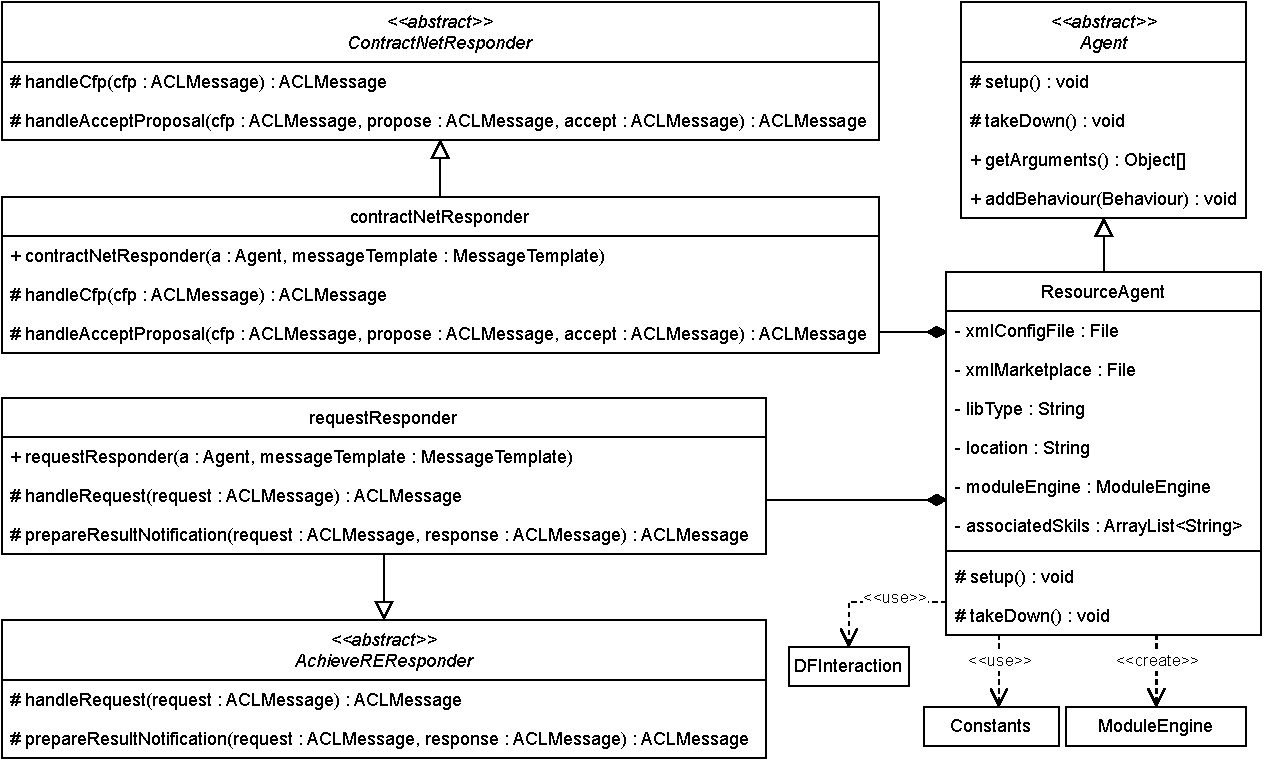
\includegraphics[scale=0.71]{RA_Class_Diagram}
	\caption{\acrlong{RA} class diagram.}
	\label{fig:ra_class_diagram}
\end{figure}

\subsection{Transport Agent}
\label{subsec:transport_agent}

Also launched by the \acrshort{DA}, the \acrlong{TA} class is very similar to the \acrlong{RA}. It also extends the "Agent" class and contains both "setup" and "takeDown" methods.

The only differences are in the variables it uses and the classes it implements. It uses the "getArguments" method provided by \acrshort{JADE} to get the parameters set by the \acrshort{DA}. It also needs the "xmlConfigFile" and the "xmlMarketplaceFile" for the same purposes, since it also makes use of the \acrshort{ME}. The String "libType" defines which \acrshort{LL} to use, like in the \acrshort{RA}, and it also has the ArrayList of Strings "associatedSkills" to hold the list of skills and an object "moduleEngine" that holds its instance of the \acrshort{ME}.

The only exception is the variable "location", since the \acrlong{TA} does not have a static location in the physical system. This class also makes use of the "Constants" and "DFInteraction" classes.

It implements a single "requestResponder" class which extends the "AchieveREResponder" class, used to respond to \acrshort{FIPA} Requests, provided by \acrshort{JADE}. This is because this agent does not make use of the \acrshort{FIPA} Contract Net, therefore does not need any of the classes that enable its use.

Figure~\ref{fig:ta_class_diagram} has a representation of its implementation. Once again the classes related to the \acrshort{ME} have been omitted.\\

\begin{figure}[h!]
	\centering
	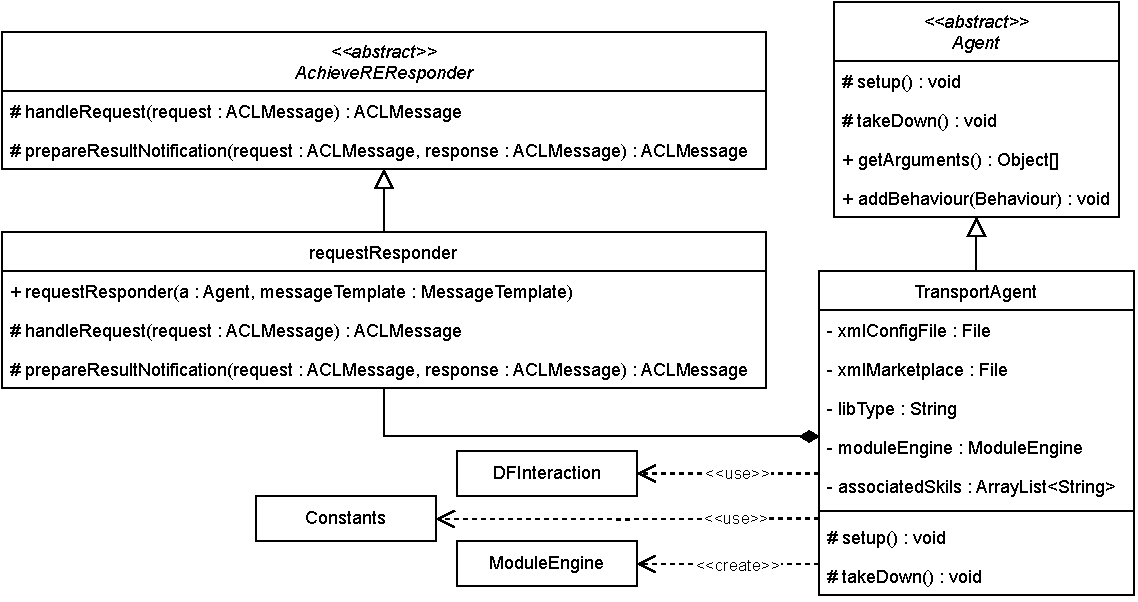
\includegraphics[scale=0.75]{TA_Class_Diagram}
	\caption{\acrlong{TA} class diagram.}
	\label{fig:ta_class_diagram}
\end{figure}

\subsection{Constants}
\label{subsec:constants}

To help define all of the constants needed for the \acrshort{MAS}, an auxiliary class of constants was created. This "Constants" class also contains a few methods to help with information retrieval. It is mostly composed of String fields. Other classes can reference it to check information about the system. All of these are implementation specific, and define the system used for testing in Chapter~\ref{cha:implementation}.\\

Figure~\ref{fig:const_class_diagram} shows a representation of this class, as it is solution specific. Generic names for each type of constant are shown to shorten the size of the diagram, with the letter "X" being used as a placeholder for names of skills, stations, products, etc. 

The Strings "SKILL\_X" define the type of skills available in the whole system. The Strings "STATION\_X" hold the \acrshort{RA} types and the "TRANSPORT\_X" holds the \acrshort{TA} types. "PROD\_X" represents the product types available. "LOCATION\_X" fields hold the value for all locations in the system. "STATION\_X\_SKILLS" and "TRANSPORT\_X\_SKILLS" list the skills those agents can perform. Finally, "PROD\_X\_SKILLS" contains the list of skills a specific product needs to complete their production and "PRODUCT\_TYPES" holds a list of all product types.\\

The methods help with information retrieval. Given an \acrshort{RA} or \acrshort{TA} name, "getStationTransportSkills" returns a list of all skills that agent is able to perform. With a name as parameter, "getStationLocation" gives the location of the station in question. "getLocationStation" does the opposite, it returns the agent name at the location passed to the method. Lastly, "getProdSkills" returns the list of skills of the product type passed as a parameter.\\

\begin{figure}[h!]
	\centering
	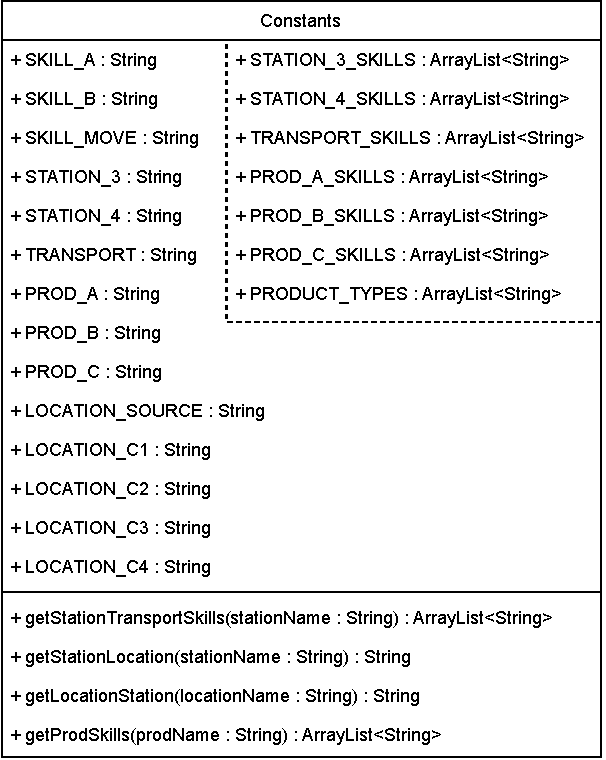
\includegraphics[scale=0.8]{Const_Class_Diagram}
	\caption{Constants class diagram.}
	\label{fig:const_class_diagram}
\end{figure}

\subsection{Directory Facilitator}
\label{subsec:directory_facilitator}

The "DFInteraction" is an auxiliary class. It provides methods that can register, remove or search information on the \acrshort{DF}, which works as a registry for agents. In it, agents can register themselves, along with the skills they provide for the \acrshort{MAS}. Other agents can then search agents by the skills they perform, and establish contact with those they find appropriate for the task, in order to request skill executions. Figure~\ref{fig:df_class_diagram} shows the diagram of the auxiliary class implementation. The method "RegisterInDF" has two version, one allows for the registry of an agent with a single skill, the other for an agent with multiple skills. The "DFService" class is implemented by \acrshort{JADE} and it is what allows for the interactions with the \acrshort{DF}.\\

\acrlongpl{RA} and \acrlongpl{TA} register themselves in the \acrshort{DF} during their setup, with the skills they are able to perform. During production, \acrlongpl{PA} can use this registry to look up agents capable of performing their needed skills, and establish contact with those agents.

\begin{figure}[h!]
	\centering
	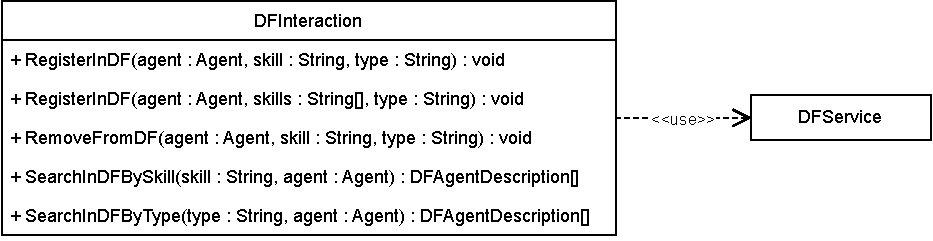
\includegraphics[scale=0.85]{DF_Class_Diagram}
	\caption{\acrlong{DF} class diagram.}
	\label{fig:df_class_diagram}
\end{figure}

\subsection{Product Manager}
\label{subsec:product_manager_agent}

The \acrfull{PM} is another deployment entity. It also presents a \acrshort{GUI} to allow a human operator to launch \acrlongpl{PA}, although it cannot terminate them. It operates similarly to the \acrshort{DA}. This class also extends the "Agent" class, and also only makes use of the "setup" method, the other functionalities called on button presses.

It generates a button per product type based on the information present in the ArrayList of Strings "productTypesList". This filed is populated by referencing the "Constants" class, which holds all the product types present in the \acrshort{MAS}. 

The "productID" is an integer appended to the name of each agent launched under the \acrshort{PM}, because \acrshort{JADE} does not allow agents with the same name to exist. The "products" ArrayList of Strings holds a list of product agents that have been launched so far.

In Figure~\ref{fig:pm_class_diagram}, the classes that it uses to draw the \acrshort{GUI} are shown, once again the "ContainerController" used to instantiate a container where \acrlongpl{PA} are launched. The "DefaultTableModel" class helps with the definition of the \acrshort{GUI}, and is a class in the "javax.swing" package.

\begin{figure}[h!]
	\centering
	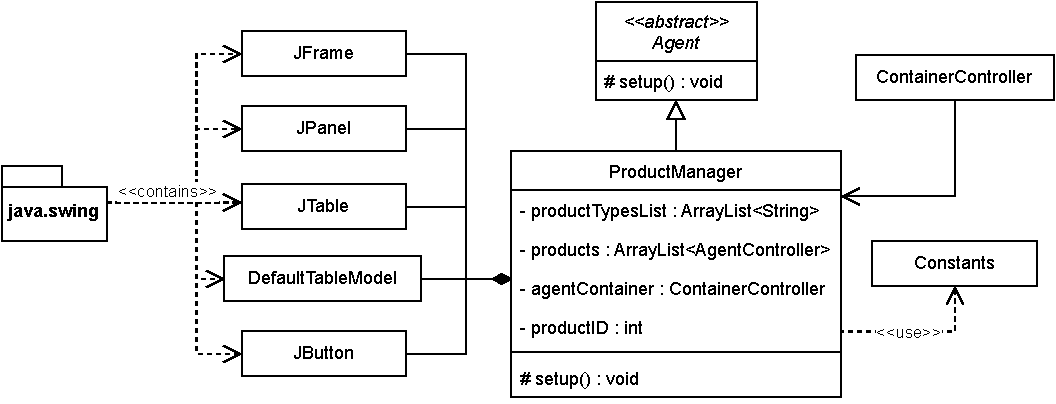
\includegraphics[scale=0.8]{PM_Class_Diagram}
	\caption{\acrlong{PM} class diagram.}
	\label{fig:pm_class_diagram}
\end{figure}

\subsection{Product Agent}
\label{subsec:product_agent}

The \acrlong{PA} class extends the "Agent" abstract class and overrides the "setup" and "takeDown" methods. It makes use of the "addBehaviour" and "getArguments" methods, as well as the "OneShotBehaviour", "ContractNetInitiator" and "AchieveREInitiator" classes. It also uses the auxiliary "Constants" and "DFInteraction" classes explained before.

It has an ArrayList of Strings called "executionPlan" to store the whole skill sequence, an int called "step" to store the current step in that sequence and a String "location" that stores the agents current location on the physical system.

The "executeNextSkill" class extends the "OneShotBehaviour" class, the "contractNetInitiator" class extends the "ContractNetInitiator" class and the "requestTransportMove" and "requestStationSkill" classes extend the "AchieveREInitator" class. These classes and methods are all represented in Figure~\ref{fig:pa_class_diagram}, along with the variables they use.

\begin{figure}[h!]
	\centering
	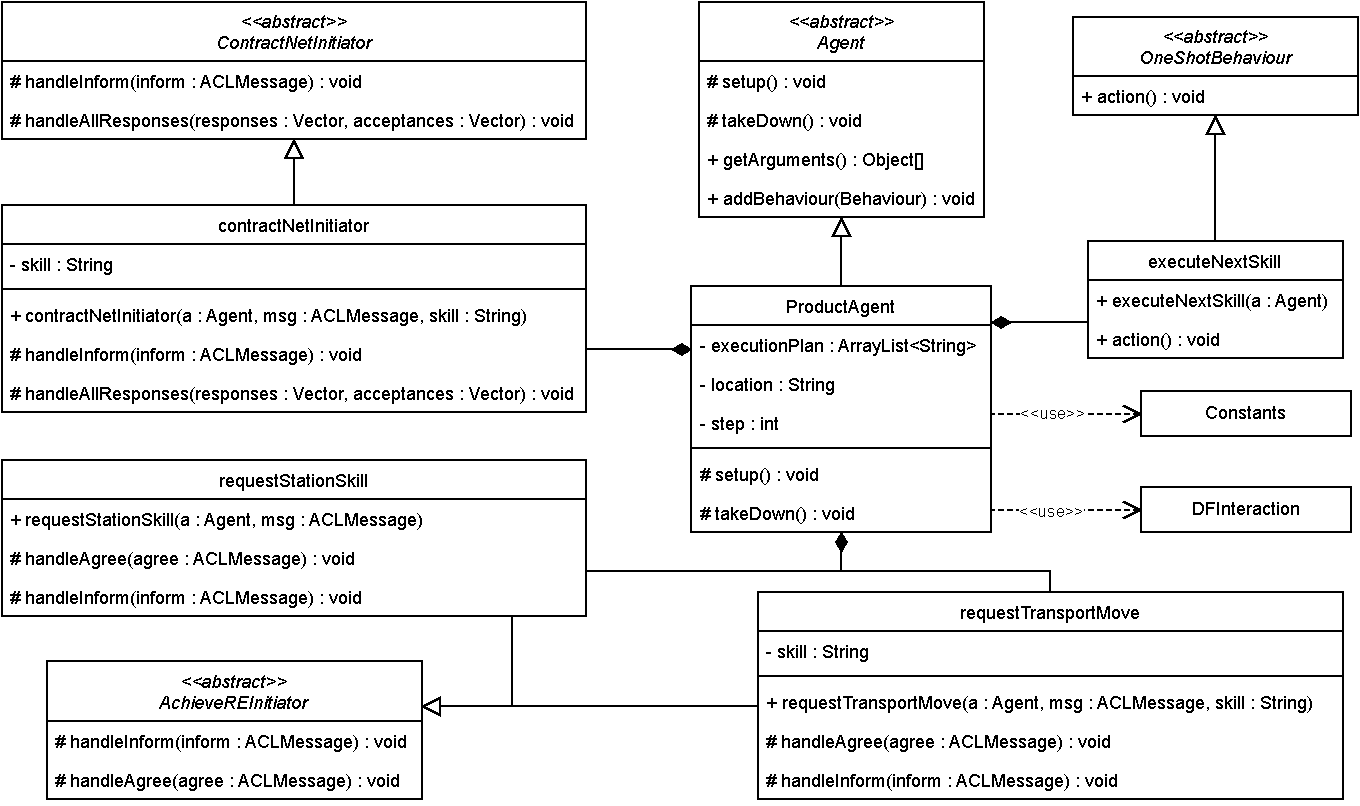
\includegraphics[scale=0.6]{PA_Class_Diagram}
	\caption{\acrlong{PA} class diagram.}
	\label{fig:pa_class_diagram}
\end{figure}

\subsection{Module Engine}
\label{subsec:module_engine}

With the whole \acrshort{MAS} already defined, the hardware interface is now going to be explained. The \acrlong{ME} class is the main framework that was developed for this. It contains a generic object "linkLibrary" that holds the currently loaded \acrlong{LL}. This object needs to be generic since, at the start of runtime, the \acrshort{ME} does not know which type of \acrshort{LL} will be loaded.

The method "parseMarketplaceXML" does exactly that, it parses the marketplace file with all the names and paths of all available \acrlongpl{LL} and places them in the "classesToLoad" Hashmap. The name is used as the key, since it is unique, and the path as the value. This marketplace file is in the \acrshort{XML} format, and holds both the name of the \acrshort{LL} and the file path of the class that implements it. Evidently, if a \acrlong{LL} has not been previously registered in the marketplace file, the \acrlong{ME} will not be able to find it, and therefore, load it. Currently, this file needs to be created and maintained by the developer, although a more complex solution could be implemented, making use of a package distribution application to download and update \acrshortpl{LL}.

These \acrlongpl{LL} are loaded inside the \acrshort{ME} by using the Reflections feature of the Java language. It allows for a program to inspect itself, and more importantly, to load classes and call their methods during runtime. This is what allows the \acrshort{ME} to load any kind of \acrshort{LL} at any point, while the \acrshort{MAS} is running. This is important, because normally all the classes Java makes use of need to be compiled. However, since the \acrshortpl{LL} that might end up being used may or may not have been created by the same developer, or exist at the time of compilation, the \acrshort{ME} needs this feature to accomplish its goal of being modular and flexible.

The method "createObject" takes the String "libType" from the agent that contains the type of \acrshort{LL} to load. This \acrshort{LL} is then fetched from the "classedToLoad" Hashmap and attributed to a generic object of type "Class", or "Class<?>". This is then loaded using Reflections by creating a new object of that class and passing along the \acrshort{XML} configurations file received from the agent as a parameter.

To execute a skill the method "executeSkill" is called with the skill as the argument, which will in turn get the method "ExecuteSkill" from the "linkLibrary" object and place it in a "Method" type object. This method is then invoked to execute the skill, which is passed to the \acrshort{LL} also as an argument, and its return message is returned as a String.

Finally, the method "shutdown" is used to disconnect the hardware from the \acrlong{LL}, and is usually called when the agent, and consequently the \acrshort{ME}, is terminated. Figure~\ref{fig:module_engine_class_diagram} shows how this class is implemented, along with an \acrshort{LL}, This one implements the \acrshort{HTTP} protocol, but it could have been any other like \acrshort{MQTT}, \acrshort{OPCUA}, etc.\\

\begin{figure}[h!]
	\centering
	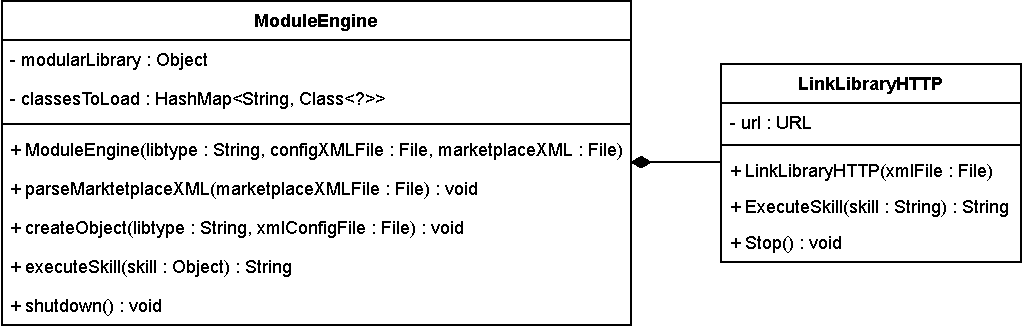
\includegraphics[scale=0.85]{ME_Class_Diagram}
	\caption{\acrlong{ME} class diagram with exemplary \acrlong{LL}.}
	\label{fig:module_engine_class_diagram}
\end{figure}

\subsection{Link Libraries}
\label{subsec:link_library_class}

To showcase the functionalities of the \acrshort{ME}, three different \acrlongpl{LL} were developed, each one implementing a different communication protocol. An abstract class "LinkLibrary" was extended to implement the "LinkLibraryHTTP", "LinkLibraryMQTT" and "LinkLibraryOPCUA" classes.

The "LinkLibraryHTTP" was implemented with the classes and methods provided in the "java.net" package. It communicates through \acrshort{HTTP} Requests. When it receives a message from the \acrshort{ME}, it will relay it to the hardware through a POST message. It will now wait until the response of this POST gets returned, with the result of the operation in it.

The "LinkLibraryMQTT" is dependent on the "org.eclipse.paho.client.mqttv3" package to implement its \acrshort{MQTT} protocol. When the \acrshort{LL} is started, it will immediately try to connect to the broker specified in its configurations, and immediately subscribe to a response topic, also present in the configurations. When a skill needs execution, the \acrshort{LL} publishes the skill in the requests topic, also specified in the configurations. Then, it will wait until the response topic receives a message, which it will return as the result to the operation.

Finally, the "LinkLibraryOPCUA" used the "org.eclipse.milo.opcua" package to implement an \acrshort{OPCUA} communication. It will connect to the \acrshort{OPCUA} server in the configuration file, and subscribe to the response node of the corresponding device. When a skill needs to be executed, the response node is cleared to make sure the result is read properly. Then the skill is written on the requests node and the \acrshort{LL} will wait until the response node value changes. When it does, the requests node is cleared, so it is ready for the next communication, and the result is returned to the agent.

All \acrlongpl{LL} must extend the "LinkLibrary" class, because this is the basis of an \acrshort{LL} and it defines the methods on which the \acrlong{ME} depends on for correct execution. All further \acrlongpl{LL} also need to take this base, to ensure correct integration with the \acrshort{ME}.

Figure~\ref{fig:link_library_class_diagram} has a representation of these classes and the respective packages they use to implement their communication protocols.\\

\begin{figure}[h!]
	\centering
	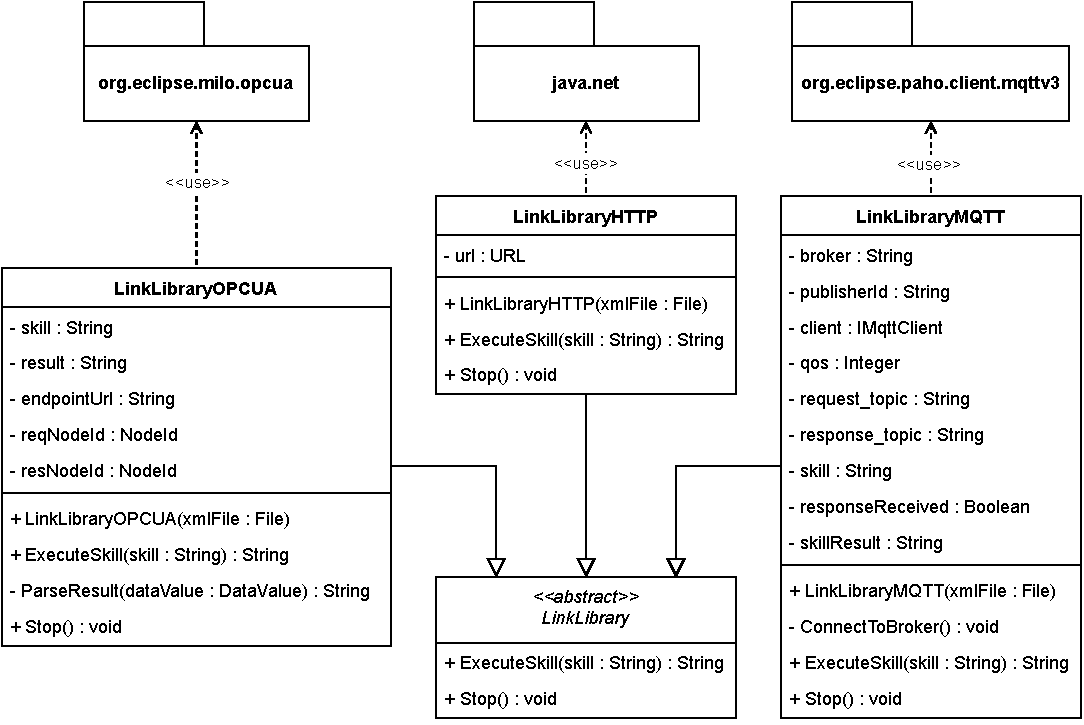
\includegraphics[scale=0.7]{LL_Class_Diagram}
	\caption{\acrlong{LL} class diagrams.}
	\label{fig:link_library_class_diagram}
\end{figure}

All developed \acrlongpl{LL} were registered in the marketplace file, one \acrshort{LL} per \acrshort{XML} tag, each tag with two attributes. The first attribute is the exact name of the class and the second attribute the file path that points to where the given \acrshort{LL} is located. With these two attributes, the \acrshort{ME} is capable of finding and loading the correct \acrshort{LL}. In order to use these \acrlongpl{LL} however, the hardware that would work underneath the agent would also need to implement these three protocols in some way. In addition, a configuration file must always be provided to the \acrshort{LL} for it to communicate properly.

\section{Interfaces}
\label{sec:interfaces}

In this Section, the three interfaces between entities in the \acrshort{MAS} are explained. Starting with the human to agent interface, for agent deployment. Then agent to agent interfaces, for \acrshort{MAS} operations. Finally, agent to hardware for skill execution.

\subsection{Human to Agent}
\label{subsec:human_to_agent_interface}

As mentioned before, there are two agents with \acrlongpl{GUI}. The \acrlong{DA} and \acrlong{PM} both present a human user with an interface for agent deployment.

On the left side the \acrshort{DA} interface has a button to open a configuration file and a text box where the path to the currently chosen file appears. Then it has a text field where the agent name is written and two radio buttons where the agent type can be selected, \acrlong{RA} and \acrlong{TA}. Finally there is a list of all available \acrshortpl{LL} that are fetched from the marketplace file and a button that starts the agent. On the right side there is a list with the currently running \acrshortpl{RA} and \acrshortpl{TA}. These agents can be selected by clicking on them and stopped by pressing the stop agent button below the list. Figure~\ref{fig:da_gui} shows this interface.\\

\begin{figure}[h!]
	\centering
	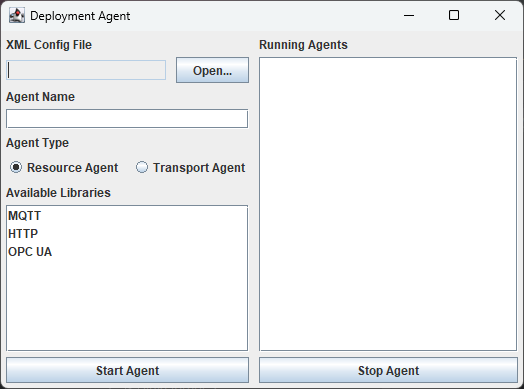
\includegraphics[scale=0.75]{DA_GUI}
	\caption{\acrlong{DA} \acrlong{GUI}.}
	\label{fig:da_gui}
\end{figure}

The \acrshort{PM} is more simple. It has buttons equivalent to the number of product agents specified in the "Constants" class and a list with the already launched agents. These agents have an ID represented by an integer, their product type and the skill sequence they need executed to complete the production process. This interface is shown in Figure~\ref{fig:pm_gui}.

\begin{figure}[h!]
	\centering
	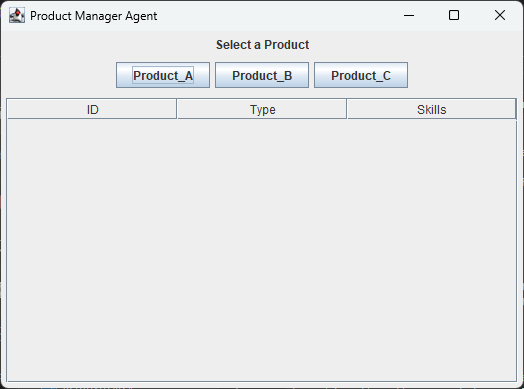
\includegraphics[scale=0.75]{PM_GUI}
	\caption{\acrlong{PM} \acrlong{GUI}.}
	\label{fig:pm_gui}
\end{figure}

\subsection{Agent to Agent}
\label{subsec:agent_to_agent_interface}

Agent to agent communication is done through ACLMessages. These have been defined by \acrshort{FIPA} \cite{FIPA_ACLMessage}. These messages have many parameters that help define communications. Table~\ref{tb:aclmessage_parameters} shows the parameters used by the agents of the \acrshort{MAS}, along with their utility.\\

\begin{table}[h!]
	\centering
	\caption{ACLMessage parameters.}
	\begin{tabular}{|c|c|}
		\hline
		Parameter    & Purpose                   \\ \hline
		performative & Type of communicative act \\ \hline
		sender       & Sender of the message     \\ \hline
		receiver     & Receiver of the message   \\ \hline
		content      & Content of the message    \\ \hline
	\end{tabular}
	\label{tb:aclmessage_parameters}
\end{table}

The performative of a message can take multiple values. For the \acrshort{FIPA} Requests protocol, messages of type "request", "refuse", "agree", "failure", "inform-done" and "inform-result". The \acrshort{FIPA} ContractNet protocol makes use of messages of type "Call For Proposals" or "CFP", "refuse", "propose", "reject-proposal", "accept-proposal", "failure", "inform-done" and "inform-result". These message types and their respective protocols can be seen in Table~\ref{tb:aclmessage_performative_types}.\\

The sender and receiver parameters are pretty self explanatory, they hold the agent ID of both the sender and receiver of the messages. The content parameter holds the content of the message. For this \acrshort{MAS} it can be a location or a skill, depending on which type of agents are communicating and at what stage a product is along its cycle.\\

\begin{table}[h!]
	\centering
	\caption{ACLMessage performative types}
	\begin{tabular}{c|cc|}
		\cline{2-3}
		\multicolumn{1}{l|}{}                 & \multicolumn{2}{c|}{Protocol}               \\ \hline
		\multicolumn{1}{|c|}{Parameter}       & \multicolumn{1}{c|}{ContractNet} 			& Requests 		\\ \hline
		\multicolumn{1}{|c|}{Request}         & \multicolumn{1}{c|}{}            			& \checkmark    \\ \hline
		\multicolumn{1}{|c|}{Refuse}          & \multicolumn{1}{c|}{\checkmark}          	& \checkmark    \\ \hline
		\multicolumn{1}{|c|}{Agree}           & \multicolumn{1}{c|}{}            			& \checkmark    \\ \hline
		\multicolumn{1}{|c|}{Failure}         & \multicolumn{1}{c|}{\checkmark}           	& \checkmark    \\ \hline
		\multicolumn{1}{|c|}{Inform-done}     & \multicolumn{1}{c|}{\checkmark}          	& \checkmark    \\ \hline
		\multicolumn{1}{|c|}{Inform-result}   & \multicolumn{1}{c|}{\checkmark}           	& \checkmark    \\ \hline
		\multicolumn{1}{|c|}{CFP}             & \multicolumn{1}{c|}{\checkmark}           	&          		\\ \hline
		\multicolumn{1}{|c|}{Propose}         & \multicolumn{1}{c|}{\checkmark}           	&          		\\ \hline
		\multicolumn{1}{|c|}{Reject-proposal} & \multicolumn{1}{c|}{\checkmark}           	&          		\\ \hline
		\multicolumn{1}{|c|}{Accept-proposal} & \multicolumn{1}{c|}{\checkmark}           	&          		\\ \hline
	\end{tabular}
	\label{tb:aclmessage_performative_types}
\end{table}

\subsection{Agent to Hardware}
\label{subsec:agent_to_hardware_interface}

To interface with the hardware, an agent must call the "executeSkill" method of the \acrlong{ME}. In its parameters it should send the skill as a String. The \acrshort{ME} will then call the "ExecuteSkill" of the \acrshort{LL} loaded by it. All \acrlongpl{LL} must contain the method "ExecuteSkill", otherwise calling it would be impossible. This method is implemented by the abstract class "LinkLibrary", as described in \ref{subsec:module_engine}.

The \acrshort{LL} will now forward the skill through the protocol it is implementing, in whatever format it was designed for. A developer could reformat this message to whatever type they want, to adapt to the hardware if needed, but the \acrshort{LL} must always return a result of type String. As long as these rules are obeyed, \acrlongpl{LL} can be used in the way most suitable to the system they are in. The result is passed to the \acrshort{ME} as a String, which is then passed to the agent.\\

Three \acrlongpl{LL} were implemented, seen in \ref{subsec:link_library_class}. The \acrshort{HTTP} \acrshort{LL} works by creating an \acrshort{HTTP} connection, every time a skill is to be executed, using the address provided in the configurations. It sends the skill as a payload in a POST request. It then waits for an OK message with code 200 as per the \acrshort{HTTP} protocol.

This response must include the result of the operation that is converted into a String and passed upward to the \acrshort{ME}. This \acrshort{LL} does not need to disconnect from the \acrshort{HTTP} server, since this protocol does not depend on a persistent connection.\\

The implemented \acrshort{MQTT} \acrshort{LL} needs more parameters to work. It requires an \acrshort{MQTT} broker address, a \acrfull{QoS} value, a request topic and a response topic. These topics are differentiated to allow for a simpler implementation of the \acrshort{LL}.

When the \acrshort{LL} is loaded, it immediately establishes a connection to the broker and subscribes to the response topic. This means that every time a response arrives, the callback function is called. This function simply stores the message as a String.

Whenever the "ExecuteSkill" method is run, the \acrshort{LL} will publish the skill in the request topic. It then waits until the response topic gets a message. Upon receiving it, it will return it to the \acrshort{ME}. When this \acrshort{LL} needs to disconnect, it just disconnects from the broker.\\

The \acrshort{OPCUA} \acrshort{LL} is a bit more complex than the other two. It also needs a server address, or endpoint, and a namespace. This namespace identifies which container the node representing the hardware is. In this node, two variable nodes are found, one for incoming requests and one for outgoing responses. To summarize, the \acrshort{LL} needs and endpoint address, a namespace, the identifier of the request node and the identifier response node.

When the \acrshort{LL} is loaded, it immediately connects to the \acrshort{OPCUA} server and creates two node objects locally with the namespace and identifiers, one with the request and one with the response identifier. It also creates a subscription to the responses node.

When a skill is to be executed, first the response node is cleared, to make sure the \acrshort{LL} gets notified of a new message. Then the skill is written to the requests node. The \acrshort{LL} waits until a response arrives and when it does it saves it and clears the requests node for the next cycle of communications. The result message is sent to the Module Engine to be returned to the agent.\\


\section{Multi-agent System Operations}
\label{sec:mas_operations}

With the whole system now defined, a review on how it operates is going to be presented. Before the system can be started, the marketplace file needs to contain the names and paths of the \acrlongpl{LL} the \acrshort{MAS} is dependent on. 

When the \acrshort{MAS} is first executed, both the \acrlong{DA} and \acrlong{PM} are launched. These agents will run their own setups. 

The \acrshort{PM} will run its "setup" method. It will look into the "Constants" class and find what \acrlong{PA} are setup there and create buttons that correspond to each \acrshort{PA}. It will setup the container where product agents will be deployed and draw the \acrshort{GUI}.

The \acrshort{DA} will also run the "setup" method. It will try to find a marketplace file and list the \acrlongpl{LL} there listed by running the "getMarketplaceLibraries" method. Then the agent container is created and the interface will be setup with it own default values and drawn to the screen. The system is now ready to launch agents.

Figure~\ref{fig:mas_operations_1} starts when the system is first executed. It shows the steps and methods until it is operational. Since no more agents are running at this point, only the \acrshort{DA} and \acrshort{PM} are shown.

\begin{figure}[h!]
	\centering
	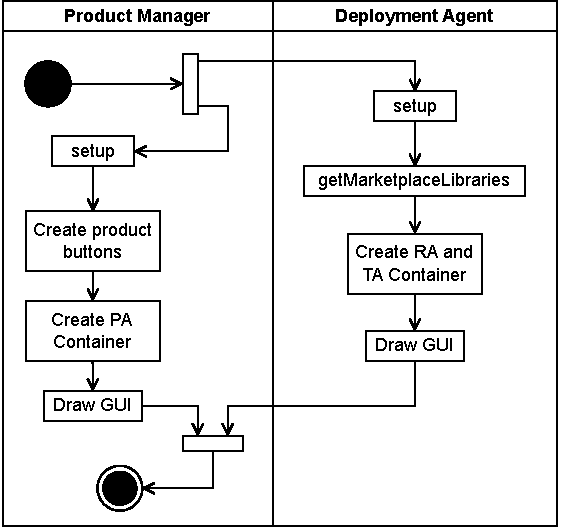
\includegraphics{MAS_Operations_1}
	\caption{\acrlong{MAS} startup.}
	\label{fig:mas_operations_1}
\end{figure}

Before any product can be produced however, a human operator needs to deploy the \acrlongpl{RA} and \acrlongpl{TA} that compose the system.\\

\subsection{Initial Setup}
\label{subsec:initial_setup}

\acrlongpl{RA} and \acrlongpl{TA} agents need to be deployed through the \acrshort{DA}. From the available \acrlongpl{LL}, the operator will chose which one needs to be launched with the agent to interface with the hardware. This \acrshort{LL} must have been previously developed according to the specifications so it is compatible with the \acrlong{ME}, and its name and file path added to the marketplace file. Upon selecting an \acrshort{LL}, the corresponding configuration file for this agent must be selected. Then the agent must be given a name and its type selected. Now the agent can be deployed by pressing the "Start Agent" button. This process now needs to be repeated for every agent, until all the agents have been launched.

When an agent is launched, its "setup" method is run. In it the agent will start the \acrshort{ME} with the \acrshort{LL} of the type selected, with the configurations provided to it. It will create a \acrlong{LL} object by getting all the \acrlongpl{LL} in the marketplace file with "parseMarketplaceXML" and create an \acrshort{LL} object with "createObject". This \acrshort{LL} will now connect to the hardware if needed, in its constructor. The agents registers itself in the \acrshort{DF} using the method "RegisterInDF". Then the first behaviour is added to the agents operating sequence. In the case of the \acrshort{RA}, it will be the "contractNetInitiator" and the "requestResponder". In the case of the \acrshort{TA}, it will only be the "requestResponder".

Figure~\ref{fig:mas_operations_2} shows this process for either a \acrlong{RA} or \acrlong{TA}. In the case of the \acrshort{RA}, the "contractNetInitiator" behaviour needs to be added as well. The \acrshort{DA} is omitted here for simplicity, since it would only deploy the agent.\\

\begin{figure}[h!]
	\centering
	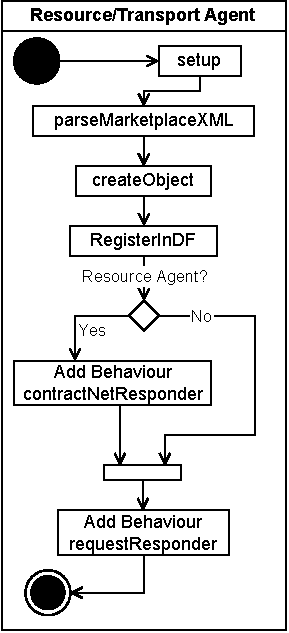
\includegraphics[scale=1]{MAS_Operations_2}
	\caption{Agent startup.}
	\label{fig:mas_operations_2}
\end{figure}

With the \acrshort{MAS} now built, new products can be launched by pressing the corresponding button in the \acrshort{PM}.

\subsection{Launching a Product}

When a product is deployed, it will get its production sequence from the \acrshort{PM} and set its own location as the starting position. It then will add the "executeNextSkill" to the behaviour sequence. This behaviour is executed immediately, its "action" method run, and it will search in the \acrshort{DF}, using "DFInteraction", for an agent capable of performing its first skill. Upon finding it, it proceeds to send a Call for Proposals to all found agents.

For this the "contractNetInitiator" class is added to the behaviours and communications are established. Upon receiving a message, the \acrshort{RA} runs "handleCfp" which generates a proposal. The \acrshort{PA} receives it in "handleAllResponses", picks one if there are multiple and answers it. "handleAcceptPorposal" from the \acrshort{RA} Informs the \acrshort{PA} of its location. Finally "handleInform" in the \acrshort{PA} looks for a transport agent in the \acrshort{DF}.

Now the product will ask the found \acrshort{TA} for transportation using the "requestTransportMove" class. This starts the \acrshort{FIPA} Requests protocol and after the \acrshort{TA} gets the first message through "handleRequest" it creates an Agree message that is forwarded to the \acrshort{PA} and immediately starts the "prepareResultNotification", which executes the skill through the \acrshort{ME} and provides a result as an inform message.\\

The \acrlong{ME}, on receiving the skill in its "executeSkill", will execute the "ExecuteSkill" method in the \acrshort{LL}. Depending on the \acrlong{LL}, the message might be sent through different channels, explained in~\ref{subsec:agent_to_hardware_interface}. When the skill finishes execution, the result is sent back to the \acrshort{TA}, which Informs the \acrshort{PA} of it completion.\\

The \acrshort{PA} now updates its location and initiates another \acrshort{FIPA} Requests communications with the class "requestStationSkill". This follows the same logic as the transportation requests, but with a \acrlong{RA} instead.

After being informed of the skills execution, the "handleInform" method increments the "step" field, which represents the execution step in the skill sequence", an checks if there are more skills to be executed. If there are, it adds a new "executeNextSkill" to the behaviour sequence and the process restarts. If there are not, the transport agent is requested again through "requestTransportMove", but this time to the deposit location in the \acrshort{MAS}, defined in the "Constants" class. After the move is complete, the agent will terminate itself.\\

In Figure~\ref{fig:mas_operations_3}, at the end of this chapter, normal system operations can be observed. The diagram specifies which class executes what method. If no class is specified then it is the agent class. The \acrshort{ME} has been initialized at this point and only needs to execute skills. All agents have been registered to the \acrshort{DF} and the \acrshort{PM} as been omitted since it would only launch the \acrlong{PA}.

\subsection{Removing Agents}

When a \acrlong{RA} or \acrlong{TA} needs to be removed from the \acrshort{MAS}, the agent needs to be selected from the \acrshort{DA} window and the "Stop Agent" button pressed. This will stop the corresponding agent by running its "takeDown" method. This method will in turn run the "shutdown" \acrlong{ME} method, which will run the "Stop" \acrshort{LL} method. 

The \acrshort{LL} will disconnect from the hardware and the agent will remove itself from the \acrshort{DF}. Finally, the agent will be terminated. This process is shown in Figure~\ref{fig:mas_operations_4}.\\

\begin{figure}[h!]
	\centering
	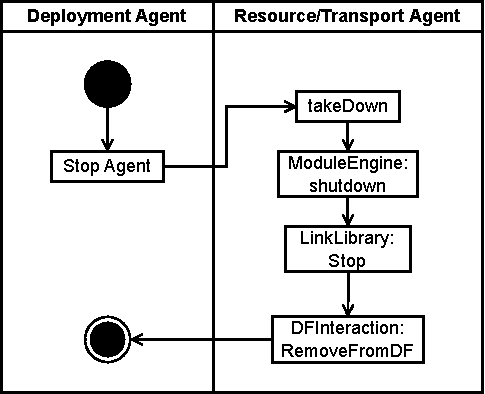
\includegraphics[scale=0.7]{MAS_Operations_4}
	\caption{Agent termination.}
	\label{fig:mas_operations_4}
\end{figure}

\begin{figure}[p]
	\centering
	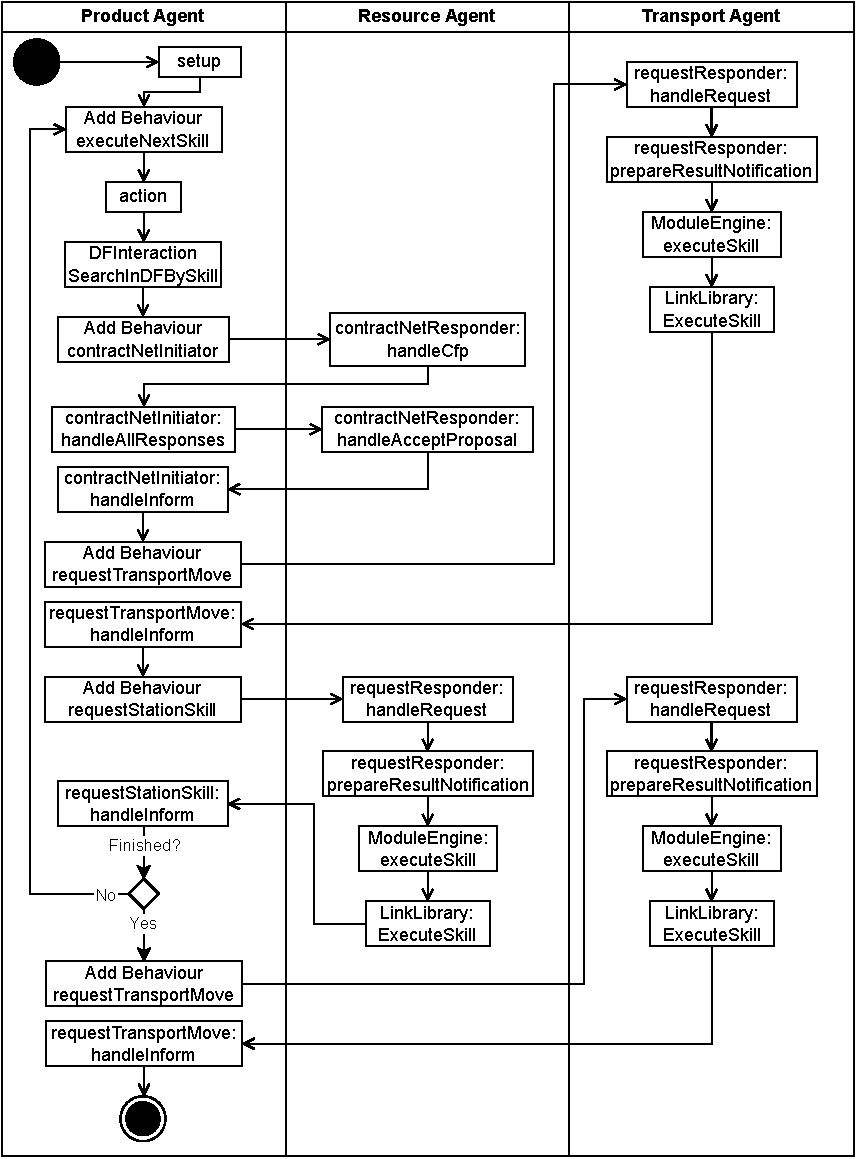
\includegraphics[scale=1]{MAS_Operations_3}
	\caption{\acrlong{MAS} operations.}
	\label{fig:mas_operations_3}
\end{figure}
